\documentclass[12pt, a4paper]{article}

\makeatletter
\begingroup\endlinechar=-1\relax
       \everyeof{\noexpand}%
       \edef\x{\endgroup\def\noexpand\homepath{%
         \@@input|"kpsewhich --var-value=HOME" }}\x
\makeatother

\def\overleafhome{/tmp}% change as appropriate
\usepackage{fontspec}
\ifx\homepath\overleafhome
\setmonofont{CONSOLA.TTF}[
BoldFont=CONSOLAB.ttf,
ItalicFont=CONSOLAI.ttf,
BoldItalicFont=CONSOLAZ.ttf
]
\else
\setmonofont{Consolas}
\fi

\usepackage[onehalfspacing]{setspace}
\parskip=1mm plus 1pt
\usepackage{indentfirst}
\usepackage{forest}
\usetikzlibrary{arrows.meta, %提供Stealth[]箭头类型
angles} %提供angle pic
	\forestset{
	tree angle/.style={
		% !表示开始相对引用。u是父节点,n是下一个兄弟节点。他们都是short-form step。
		% pic {angle}: draw a small picture of type angle.
		% angle是来自\usetikzlibrary{angles}。
		% The angle pic draws an angle between the two lines BA and BC, where A, B, and C are three coordinates.
		tikz={\path () coordinate (A) -- (!u) 
			coordinate (B) -- (!n) 
			coordinate (C) pic [draw, angle radius=#1] {angle};}
	},
	tree angle/.default=5mm
}

\usepackage[section]{placeins}

\usepackage{xcolor}
\usepackage{algorithm}
\usepackage{algorithmic}
\usepackage{hyperref}
\hypersetup{
unicode=true,          % non-Latin characters in Acrobat’s bookmarks
pdftitle={},    % title   
%pdfauthor={爱让一切都对了},     % author   
%pdfcreator={爱让一切都对了},
%pdfproducer={OpenOffice.org 3.3},
breaklinks=true,
colorlinks=true,       % false: boxed links; ture: colored links
linkcolor=blue,          % color of internal links   
citecolor=blue,        % color of links to bibliography  
filecolor=magenta,      % color of file links   
urlcolor=cyan,           % color of external links  
}
\usepackage{xcolor}

\usepackage{url}
\def\UrlBreaks{\do\A\do\B\do\C\do\D\do\E\do\F\do\G\do\H\do\I\do\J\do\K\do\L\do\M\do\N\do\O\do\P\do\Q\do\R\do\S\do\T\do\U\do\V\do\W\do\X\do\Y\do\Z\do\[\do\\\do\]\do\^\do\_\do\`\do\a\do\b\do\c\do\d\do\e\do\f\do\g\do\h\do\i\do\j\do\k\do\l\do\m\do\n\do\o\do\p\do\q\do\r\do\s\do\t\do\u\do\v\do\w\do\x\do\y\do\z\do\0\do\1\do\2\do\3\do\4\do\5\do\6\do\7\do\8\do\9\do\.\do\@\do\\\do\/\do\!\do\_\do\|\do\;\do\>\do\]\do\)\do\,\do\?\do\'\do+\do\=\do\#}

\usepackage{listings}
\lstset{
%  %行号
%  %numbers=left,
%  %背景框
%  %framexleftmargin=10mm,
%  %frame=none,
%  %背景色
%  %backgroundcolor=\color[rgb]{1,1,0.76},
%  %样式
  keywordstyle=\color{blue}\bfseries,
%  identifierstyle=\bf,
%  numberstyle=\color[RGB]{0,192,192}, %行号的样式
  commentstyle=\it\color[RGB]{0,96,96},
  stringstyle=\rmfamily\slshape\color[RGB]{128,0,0},
%  %显示空格
%  %showstringspaces=false,
  basicstyle=\ttfamily\footnotesize, %修正大写字母间距过小
  columns=flexible, %修正大写字母间距过小
  breaklines=true, %对过长的代码自动换行
%  escapechar=!,
%  morekeywords={BEGIN}
    upquote=true,
  language=python
}

\newcommand{\code}[1]{\texttt{#1}}

\title{CS 188 Security Evaluation on Team Random's Project}
\author{Weikeng Yang\\405346443 \and
Yingzhe Hu\\505366341 \and
Qiqi Gu\\604253019 \and
Dongyao Liang\\705313832 \and
Shuhua Zhan\\705190671}
\date{Team name: Random\\[2mm]February 28, 2020}

\usepackage[numbers]{natbib}
\setcitestyle{square}

\usepackage{graphicx}

\begin{document}

\maketitle

\section{Summary}




\section{Evaluation Plan}

We plan to evaluate two parts of project Google Play Advanced Search, namely the source code, and the application deployed to Google Cloud, accessible via \url{https://beta.gqqnbig.me/}. We will check the security issues in the source code, and find if the server is properly protected.

\subsection{Evaluate Source Code}
To evaluate the source code, we first revisit the design document, find any oversights as the professor mentioned our design document misses many potential risks.

When we were developing the project, we were already performing code review, ie. a team member creates pull requests (PR) for his/her changes, and an experienced team member will review the commits in the pull requests, approve the PR or request revisions. However, it is mainly Qiqi and Dongyao who review pull requests. We will ask other team members to read the code in hope that they find out something the PR reviewer missed before.

When we are doing security evaluation code review, candidate point strategies.

We will also check the security vulnerabilities of the dependencies of the project.


\subsection{Evaluate Server}
To evaluate the server, we use varies tools:

\subsubsection{Nmap}
We use Nmap to scan the open ports on our server. Currently we have a public ip \textcolor{green}{35.236.119.106} and domain beta.gqqnbig.me

Running Nmap with -F flag to scan 100 most frequently used ports.
We find these ports are open:
\begin{center}
    \begin{tabular}{l l l}
        PORT & STATE & SERVICE \\
        22/tcp & open & ssh\\
        80/tcp & open & http\\
        443/tcp & open & https
    \end{tabular}
\end{center}
These are exactly all ports we need to use. We didn't leave any unused port open.

\subsubsection{OWASP ZAP}
ZAP is a open source project developed by OWASP. It can help us to find the some potential security problems of our web server like SQL injection, XSS and many others.
We run zap to attack our website and found some Alerts:
\begin{itemize}
    \item Risk: \textcolor{orange}{low}. Cross-Domain JavaScript Source File Inclusion. We are using some third-party javascript libraries. They are:
    \begin{itemize}
        \item jQuery API:\\ \textcolor{blue}{<script src="https://code.jquery.com/jquery-3.4.1.min.js"></script>}
        \item A CDN for npm - lodash:\\ \textcolor{blue}{<script src="https://cdn.jsdelivr.net/npm/lodash@4.17.15/lodash.min.js"></script>}
        \item A progressive javascript framework - Vue.js:\\ \textcolor{blue}{<script src="https://cdn.jsdelivr.net/npm/vue@2.6.11"></script>}
    \end{itemize}
    \item Risk: \textcolor{orange}{low}. Incomplete or No Cache-control and Pragma HTTP Header Set
    \item Risk: \textcolor{orange}{low}. X-Content-Type-Options Header Missing on file \code{static/js/vue-click-outside.js} and \code{static/images/question.png}
    \item Risk: \textcolor{blue}{Informational}. Information Disclosure - Suspicious Comments
    \item Risk: \textcolor{blue}{Informational}. Timestamp Disclosure - Unix
\end{itemize}
One way to work around the first alert is by deploying the production mode of above third party javascript libraries to reduce the potential threat if we have more time.

%To evaluate the server, we want to use web security evaluation tools, including port scanners.


%scan through each possible problem areas (SQL injection attacks, XSS? --no, error handling - return code)

\section{Design Review}
\begin{figure}[ht]
\centering
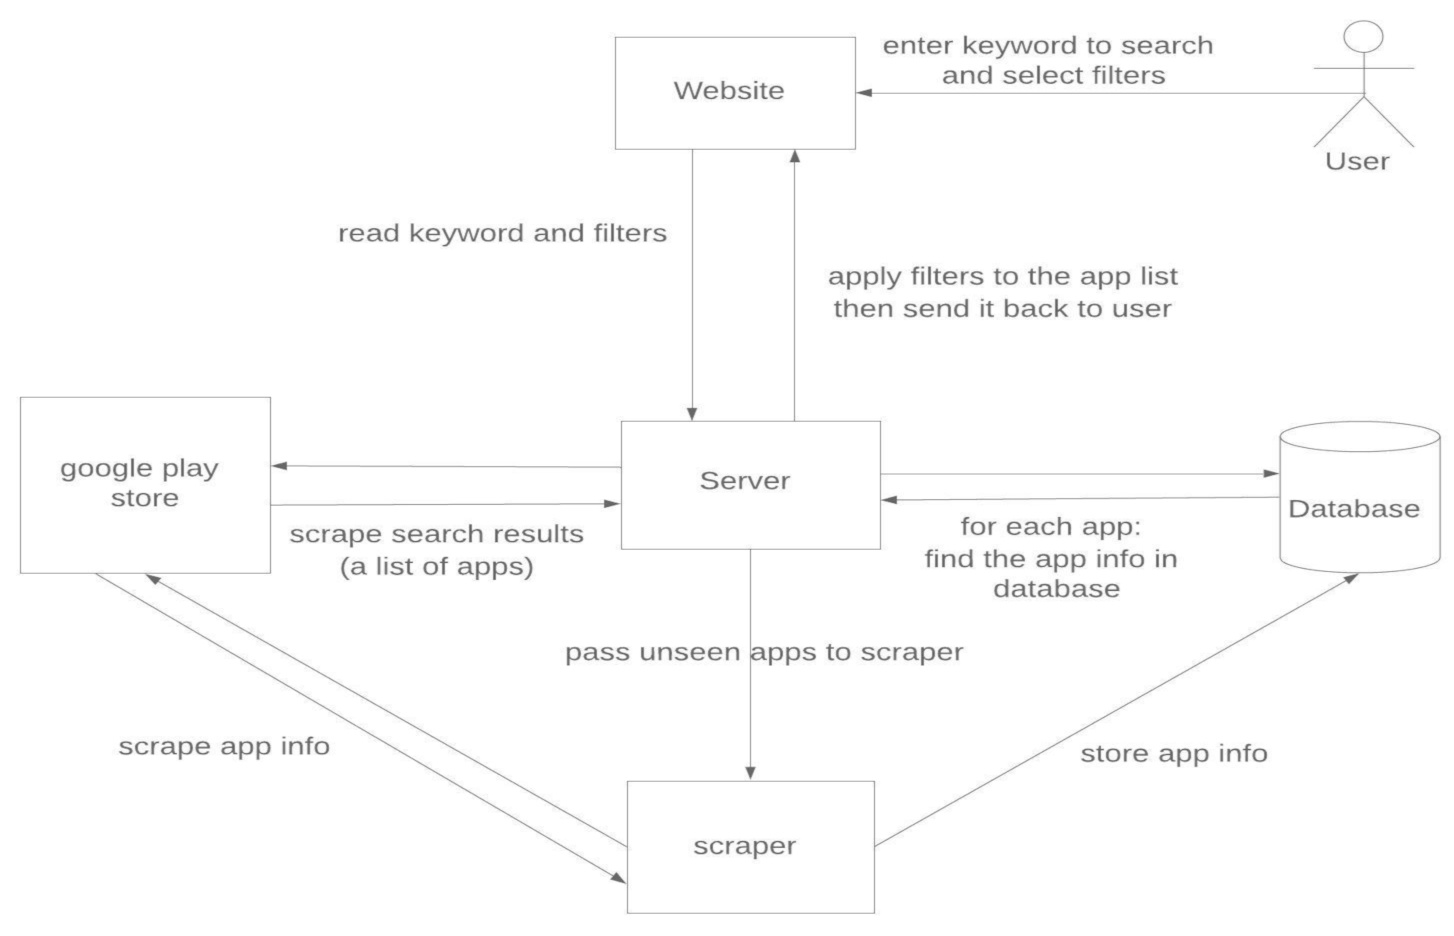
\includegraphics[width=\textwidth]{Context_Diagram.jpeg}
\caption{Design Diagram}
\label{fig:design_diagram}
\end{figure}

Figure \ref{fig:design_diagram} is the design diagram. We evaluate the design again. By looking at the source code at a high level, we conclude the implemented project largely matches the design, with a few exceptions.

\begin{figure}[ht]
\centering
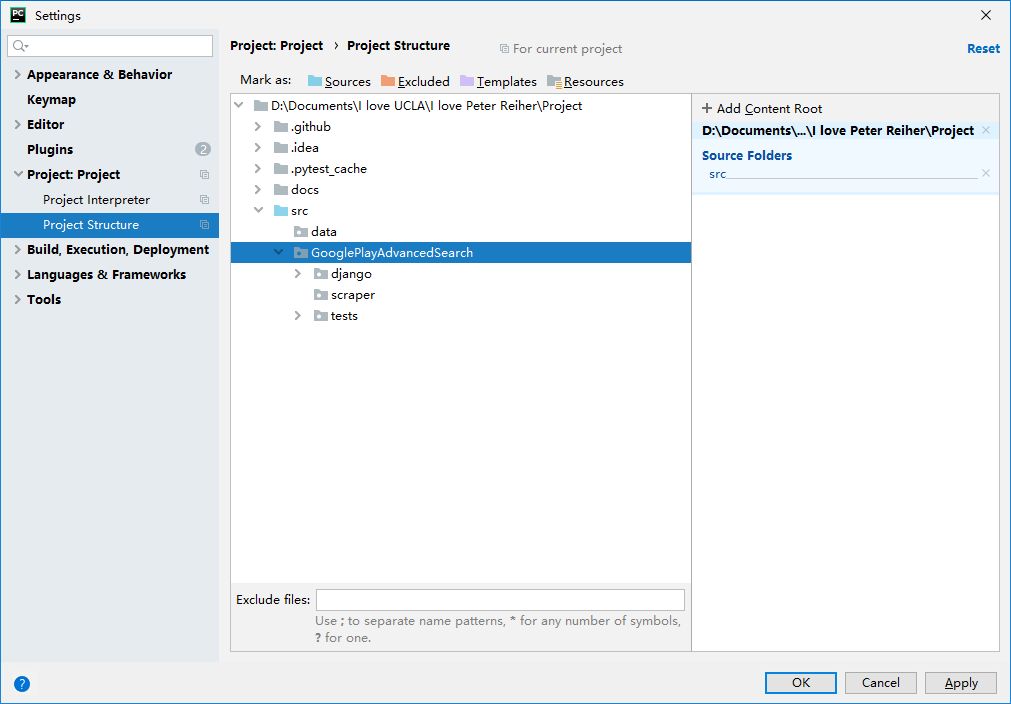
\includegraphics[width=\textwidth]{project-structure.png}
\caption{Project structure. \code{src} is the source code root.}
\label{fig:project-structure}
\end{figure}

The implemented project has 3 modules, well organized into a hierarchical namespace, see Figure \ref{fig:project-structure}. \code{src} is the source code root. tests is the additional module but since it's for automated tests, the addition is not a big deal.

The design diagram indicates there is a server component, but actually the django module and the scraper module both run on a server; the SQLite database is on the same server as well. Some functions, for instance \code{src/GooglePlayAdvancedSearch/DBUtils.py} are shared across modules. 

Unlike the design diagram, the implemented website talks to database, and run scraper as a standalone process. Both are found in \linebreak[4]
\code{GooglePlayAdvancedSearch\linebreak[0].django.web.Api}\footnote{All code are in namespace \code{GooglePlayAdvancedSearch}. Moveing forward, we will remove this prefix for conciseness and only say \code{django.web.Api}.}.

Moreover, the django module has some scraping abilities. It scrapes Google Play search result page, and if the module requires more information, it then calls scraper.

By looking at the design, we hold the threats to the application are: 1) Attackers attacking through the website; 2) Attackers attacking the server; 3) Malicious data injected from Google Play. There are also threats to end users: 4) Attackers may perform man-in-the-middle attack. 5) We have to prevent cross-site attack, and 6) check client side security vulnerabilities, mainly JavaScript.

We assign high priority to 1), 5); medium to 4), 6), low to 2), 3).

% data flow 
\begin{figure}[ht]
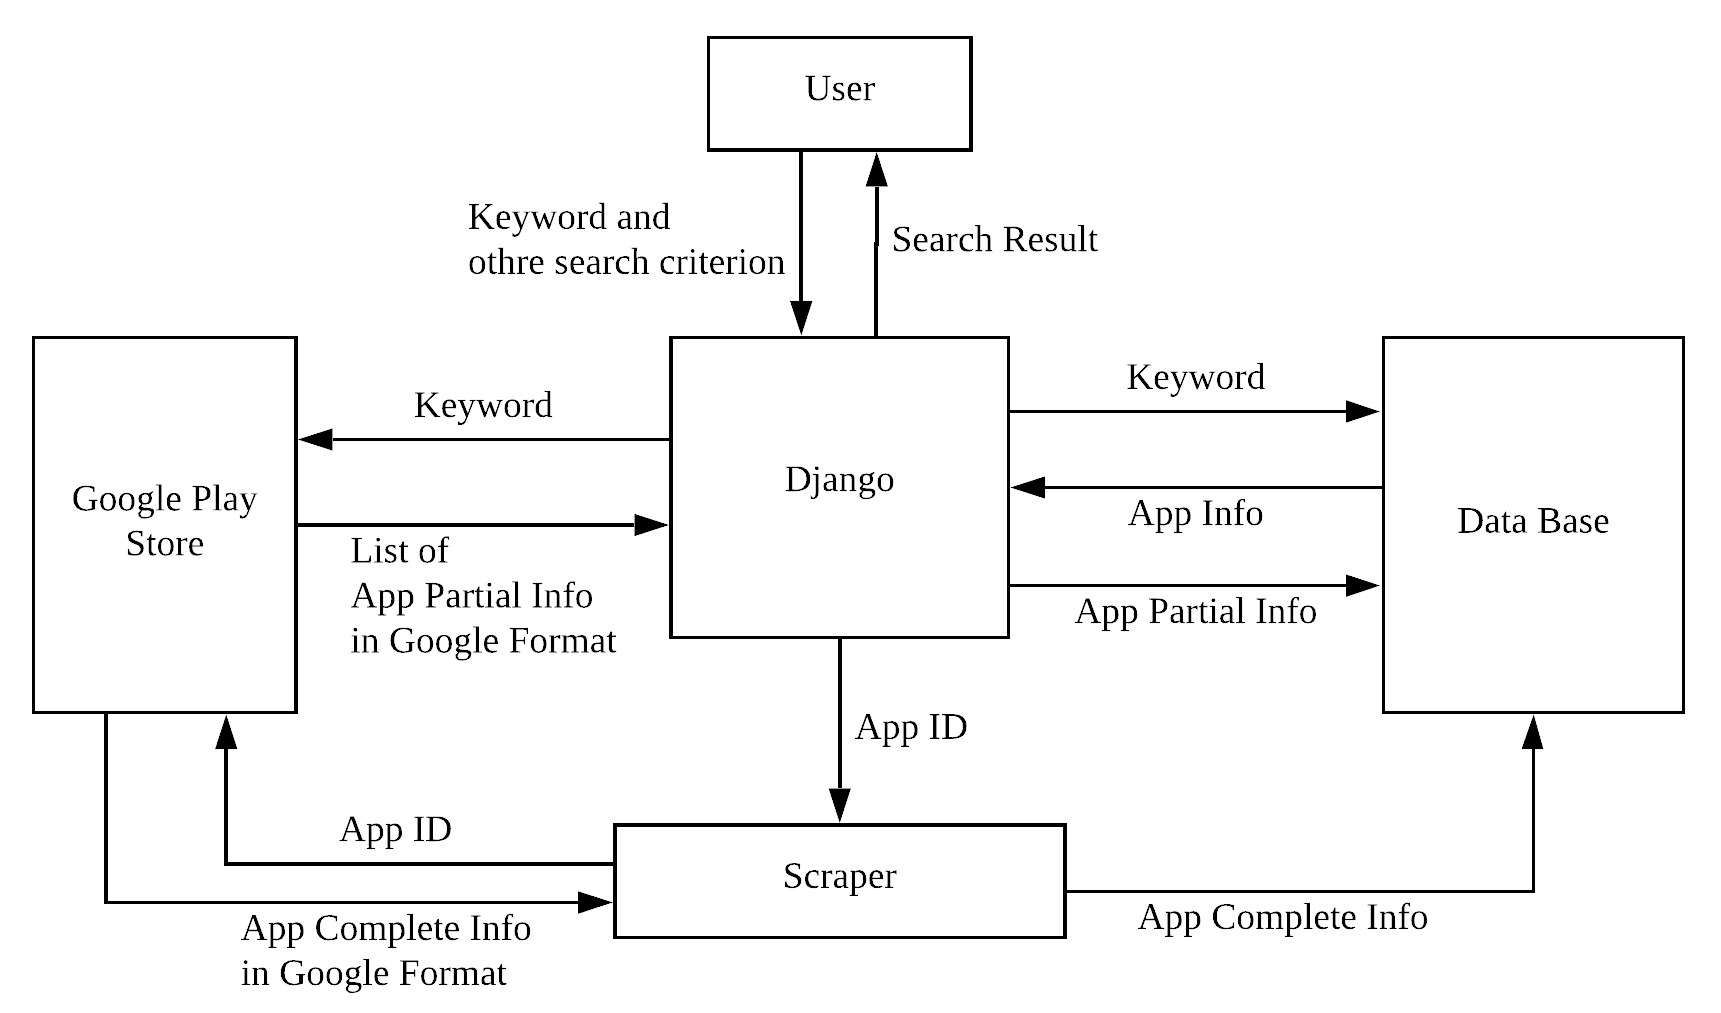
\includegraphics[width=\textwidth]{dataFlow.png}
\caption{Data Flow Diagram}
\label{fig:dataFlow}
\end{figure}

Additional, we also check and review the process of data flow. When an user uses our website(Google Play Advanced Search) to search some specific Apps, the data flow will show as the diagram. 1) Django sends the request to Google Play Store based on the user's search keywords and gets the partial information of apps back(Apps ID). 2) Django sends all the apps ID and the filtering information for user to database and try to get corresponding complete information of apps. 3) If Django makes sure that our database have all the information of apps which are searched from Google Play Store, it just return the results to the user directly. 4) Otherwise, Django will record the missing apps ID and pass them to Scraper. 5) Scraper goes to Google Play Store to get complete information of the missing apps and save all the new data in database. 6) Finally, Django grabs all the complete information from database and returns them to user.

Based on the process of data flow, we found that the most likely security issues - trace malicious input. We try to do some fuzz testings. 

\code{requirements.txt} lists the Python packages not developed by us. In addition, we use SQLite database and some client-side JavaScript libraries. Section \ref{dependency-evaluation} evaluates the security of these dependencies.


\section{Code Review}

code review approach
top down? bottom up?
While reviewing our codes, we performed top-down approach where we start with the general framework of the codes and then look deeper into specific functions.

We used Candidate point strategies, searching for \code{StringAgg(delimiter)}, which is subject to SQL injection.



% https://developer.mozilla.org/en-US/docs/Learn/Server-side/Django/web_application_security

We are running Django as our framework, so it is good to know about the protection and potential threats provided by Django.
\begin{itemize}
    \item Cross site scripting(XSS). Django's template system protects us against the majority of XSS attacks by escaping specific characters that looks dangerous in HTML. For example the string "<script>" will be turned into "\textcolor{blue}{\&lt}script\textcolor{blue}{\&lt}".
    \item Django provides some CSRF protection by invoking \code{\{\% csrf\_token \%\}} tag into form definition although we don't have any form requests.
    \item SQL injection protection. Django’s querysets are protected from SQL injection since their queries are constructed using query parameterization. A query’s SQL code is defined separately from the query’s parameters. In additional, we have written some raw queries and we need to make sure they are secure from SQL injection (we will talk about it below)
    \item Django can be configured to enforce SSL. With enabling SSL, we can use \code{SECURE\_PROXY\_SSL\_HEADER} to check if the incoming content is secure; \code{SECURE\_SSL\_REDIRECT} to redirect all http to https, (we configure a non-https to https redirection on nginx in our production server instead); and \code{SESSION\_COOKIE\_SECURE} to make sure cookies are only sent over http and \code{SESSION\_COOKIE\_SECURE} to make sure cookies are only sent over https.
\end{itemize}


We looked at the SQL injection possibility on the search box. The handler of the request is at \code{django.web.Api.search()}. We notice the user input keyword is passed into two places, namely \code{DBUtils.AppAccessor.\linebreak[0]searchApps()} and \code{django.web.Api.searchGooglePlay()}. Listing \ref{lst:searchApps} is an extract of \code{django.web.Api.searchGooglePlay()}, where a severe denial of service issue exists.

\begin{lstlisting}[frame=tb, caption=DBUtils.AppAccessor.searchApps(), label=lst:searchApps]
def searchApps(self, namePattern: str) -> List[AppItem]:
	appList = []

	self.__cursor.execute("SELECT id,name,rating,num_reviews,install_fee,inAppPurchases,app_icon FROM App WHERE name LIKE :namePattern", {"namePattern": '%' + namePattern + '%'})
\end{lstlisting}

Neither the searchApps function or the call sites verifies the length of parameter namePattern. Initially on the website, user has to type something to make the search button enabled, which might be the safe guard against searching for an empty keyword, see Figure \ref{fig:website-gray-buton}. However, if the user deletes the keyword, the search button is still enabled. Therefore user is able to search for an empty keyword, and the SQL statement doesn't limit the return rows. If there are many data in database, all data will be returned, and the execution time might be long. It can potentially become a denial of service.


\begin{figure}[ht]
\centering
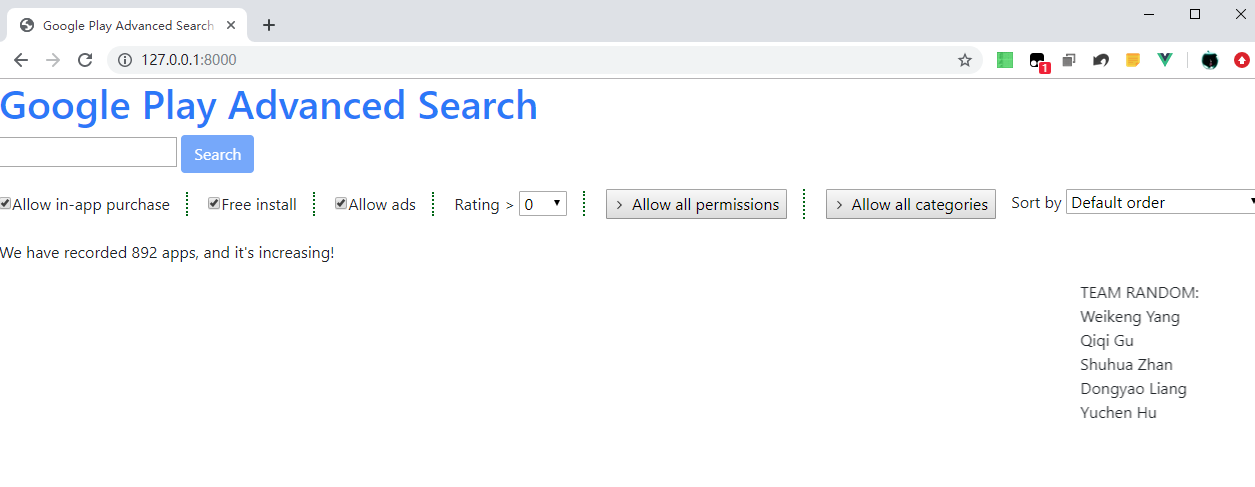
\includegraphics[width=\textwidth]{website-gray-button.png}
\caption{Initially the website has a disabled search button, but user can type something then delete them, enabling searching for empty keyword.}
\label{fig:website-gray-buton}
\end{figure}

\subsection{Automated Tests}
Project Google Play Advanced Search comes with a number of automated tests located in the tests module. These are all functional tests and the badge on the README file on the repository confirms the code passes all tests. However, there are no security tests there.




\section{Future Evaluations}
Other Python 3.7 vulnerabilities are not immediately relevant to our project because we are not using the affected functions. We should check if the dependencies are using them, but due to time constraint, we didn't do.


\section{The purpose of the software}
The project is a website searching apps on Google Play. The purpose of the software is to enhance the searching and filtering functions on Google Play so that users are able to filter apps by their permissions, whether they have ads, whether they have in-app purchase, free or paid, etc. Further, our website is able to sort apps by the number of permissions, price, stars, downloads, and sort of metrics to facilitate use case “search free sqlite database app with no ads with only storage read/write permissions, sorted by rating”.



\section{Components}
\subsection{Web Scraper}
Web Scraper is currently implemented with the help of the Python scrapy package\textsuperscript{\cite{scrapy}}. scrapy is a web scraper framework that uses Twisted reactor\textsuperscript{\cite{reactor}} to handle event loops because scrapy has events like parse response, \code{permissions\linebreak[2]\_retrieved}, \code{process\_item}, \code{open\_spider}, etc.

\code{AppInfoSpider.parse} is an event raised with parameter \code{response}, which is the HTML source code of the app detail page on Google Play. We choose proper CSS selectors or XPath selectors to scrape the app information. For instance, CSS selector \code{h1[itemprop=name]} selects the app name "Sonic the Hedgehog™ Classic" on \url{https://play.google.com/store/apps/details?hl=en&id=com.sega.sonic1px}.

SQLite3 support is part of python3 standard library.\textsuperscript{\cite{python-sqlite}}For simplicity, we choose to use sqlite3 as our database. Its query parameterization only works for the \code{where} clause.\textsuperscript{\cite{sqliteC++}}

\begin{figure}[ht]
\centering
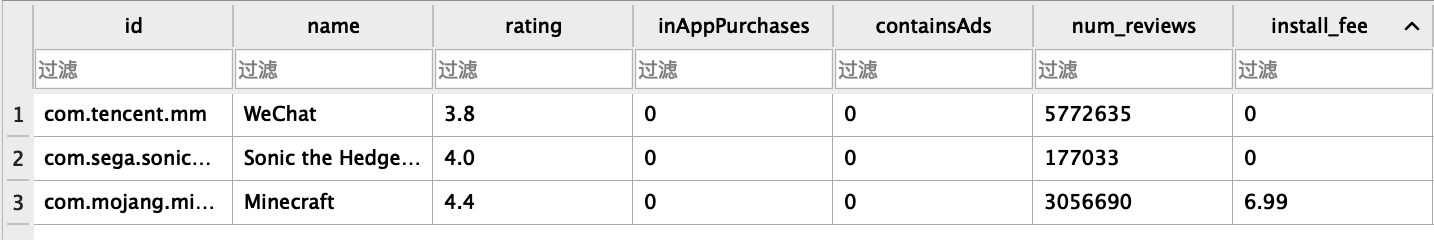
\includegraphics[width=0.8\textwidth]{critical_information.png}
\caption{Table Rows and Columns in SQLite}
\label{fig:critical-information}
\end{figure}

For now, our team has scraped 5 elements of information from Google Play Website, which are \code{rating}, \code{inAppPurchases}, \code{containAds}, \code{num\linebreak[4]\_reviews}, \code{install\_fee}, and a list of permissions. \code{rating} indicates the rating score of the apps; \code{inAppPurchases} indicates whether users are required to purchases products or pay fees inside the apps; \code{containAds} returns whether or not the apps have advertisements; \code{num\linebreak[2]\_reviews} returns the review comments from Google Play for the specific searched app; \code{install\_fee} returns the price of the apps and if it’s free, the value would be 0. Permissons are dynamically added to our table as a new column if we have never seen it before because we don't know all permissions an app can possibly have. Value of the permission columns would be 1 or 0, indicating if an app needs that permission.

\subsection{Website}
The website is built with python package Django\textsuperscript{\cite{django}}. Listing \ref{lst:pattern-matching} is Django URL pattern matching code that says if the path of the URL is empty, eg. \url{http://localhost:8080/}, the request shall be handled by \code{view.index()}. Once user submits a search request, in the proper request handler, we will use the keyword to search our database, or ask the scraper to update the database from Google Play, then return the result.

\begin{lstlisting}[frame=tb, caption=urls.py, label=lst:pattern-matching]
urlpatterns = [
    url(r'^$', view.index),
]
\end{lstlisting}

The website doesn't need to modify the database. Ideally it should open the database in read-only mode, but Django doesn't support this. Considering the data in our database are not confidential, we are fine with opening the SQLite database with full permission.



Use case:

\begin{enumerate}
    \item An user wants to search an boat game. He will type in keyword “boat”, select “Game” category and add the filters he wants (eg. free, rating>4.5, no Ads...)
    \item Our server uses the keyword and category to send a request to Google play store.
    \item Google play store will response us with a page that has a list of apps that match the keyword and the category. 
    \item we grab the app urls, then run the logic in Listing \ref{fig:database-step}.
    \item apply filters
    \item send back the filtered app list to user (see figure  \ref{fig:search_result}).
\end{enumerate}

\begin{algorithm}
    \caption{Pseduo-code for after searching an app}
    \label{fig:database-step}
\begin{algorithmic}
    \FOR{each app}
    \IF{app in our database}
    \STATE read app information
    \ELSE
    \STATE run our AppInfoSpider to scrape the app information from google play store
    \STATE put it in database
    \ENDIF
    \ENDFOR
\end{algorithmic}
\end{algorithm}
    

\begin{figure}[ht]
\centering
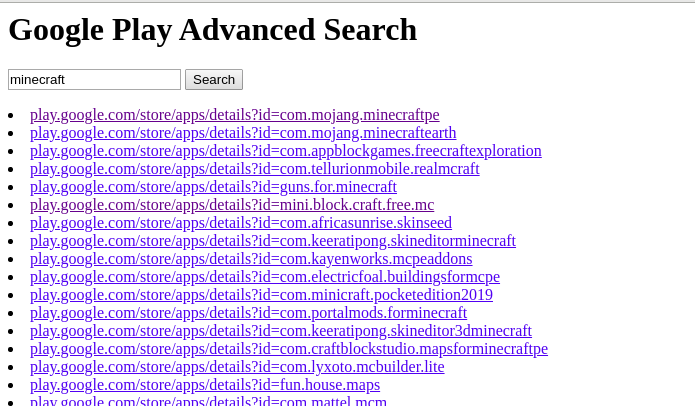
\includegraphics[width=1\textwidth]{homepage.png}
\caption{search result}
\label{fig:search_result}
\end{figure}

\section{Hardware and Software}
\subsection{Hardware}
We will rent a server from Google Cloud with reasonable storage and cores to host our application.

\subsection{Software}
The web scraper and the website are written in Python 3.7, as Python 2 is out of official support. The database is SQLite3 for now. The external python packages are recorded in \code{requirements.txt}, as seen in Listing \ref{lst:packages}.

We checked on \url{https://www.cvedetails.com/version/240190/Python-Python-3.7.html} that Python 3.7 has no major security issues.

\lstinputlisting[language={},frame=tb, caption=requirements.txt, label=lst:packages]{
\ifx\homepath\overleafhome
requirements.txt
\else
../../requirements.txt
\fi}

The whole piece of the software is runnable on both Linux and Windows system, but we will deploy it on Ubuntu 18.04 LTS.


\section{Security Requirements and Issues}

\begin{figure}[ht]
\centering
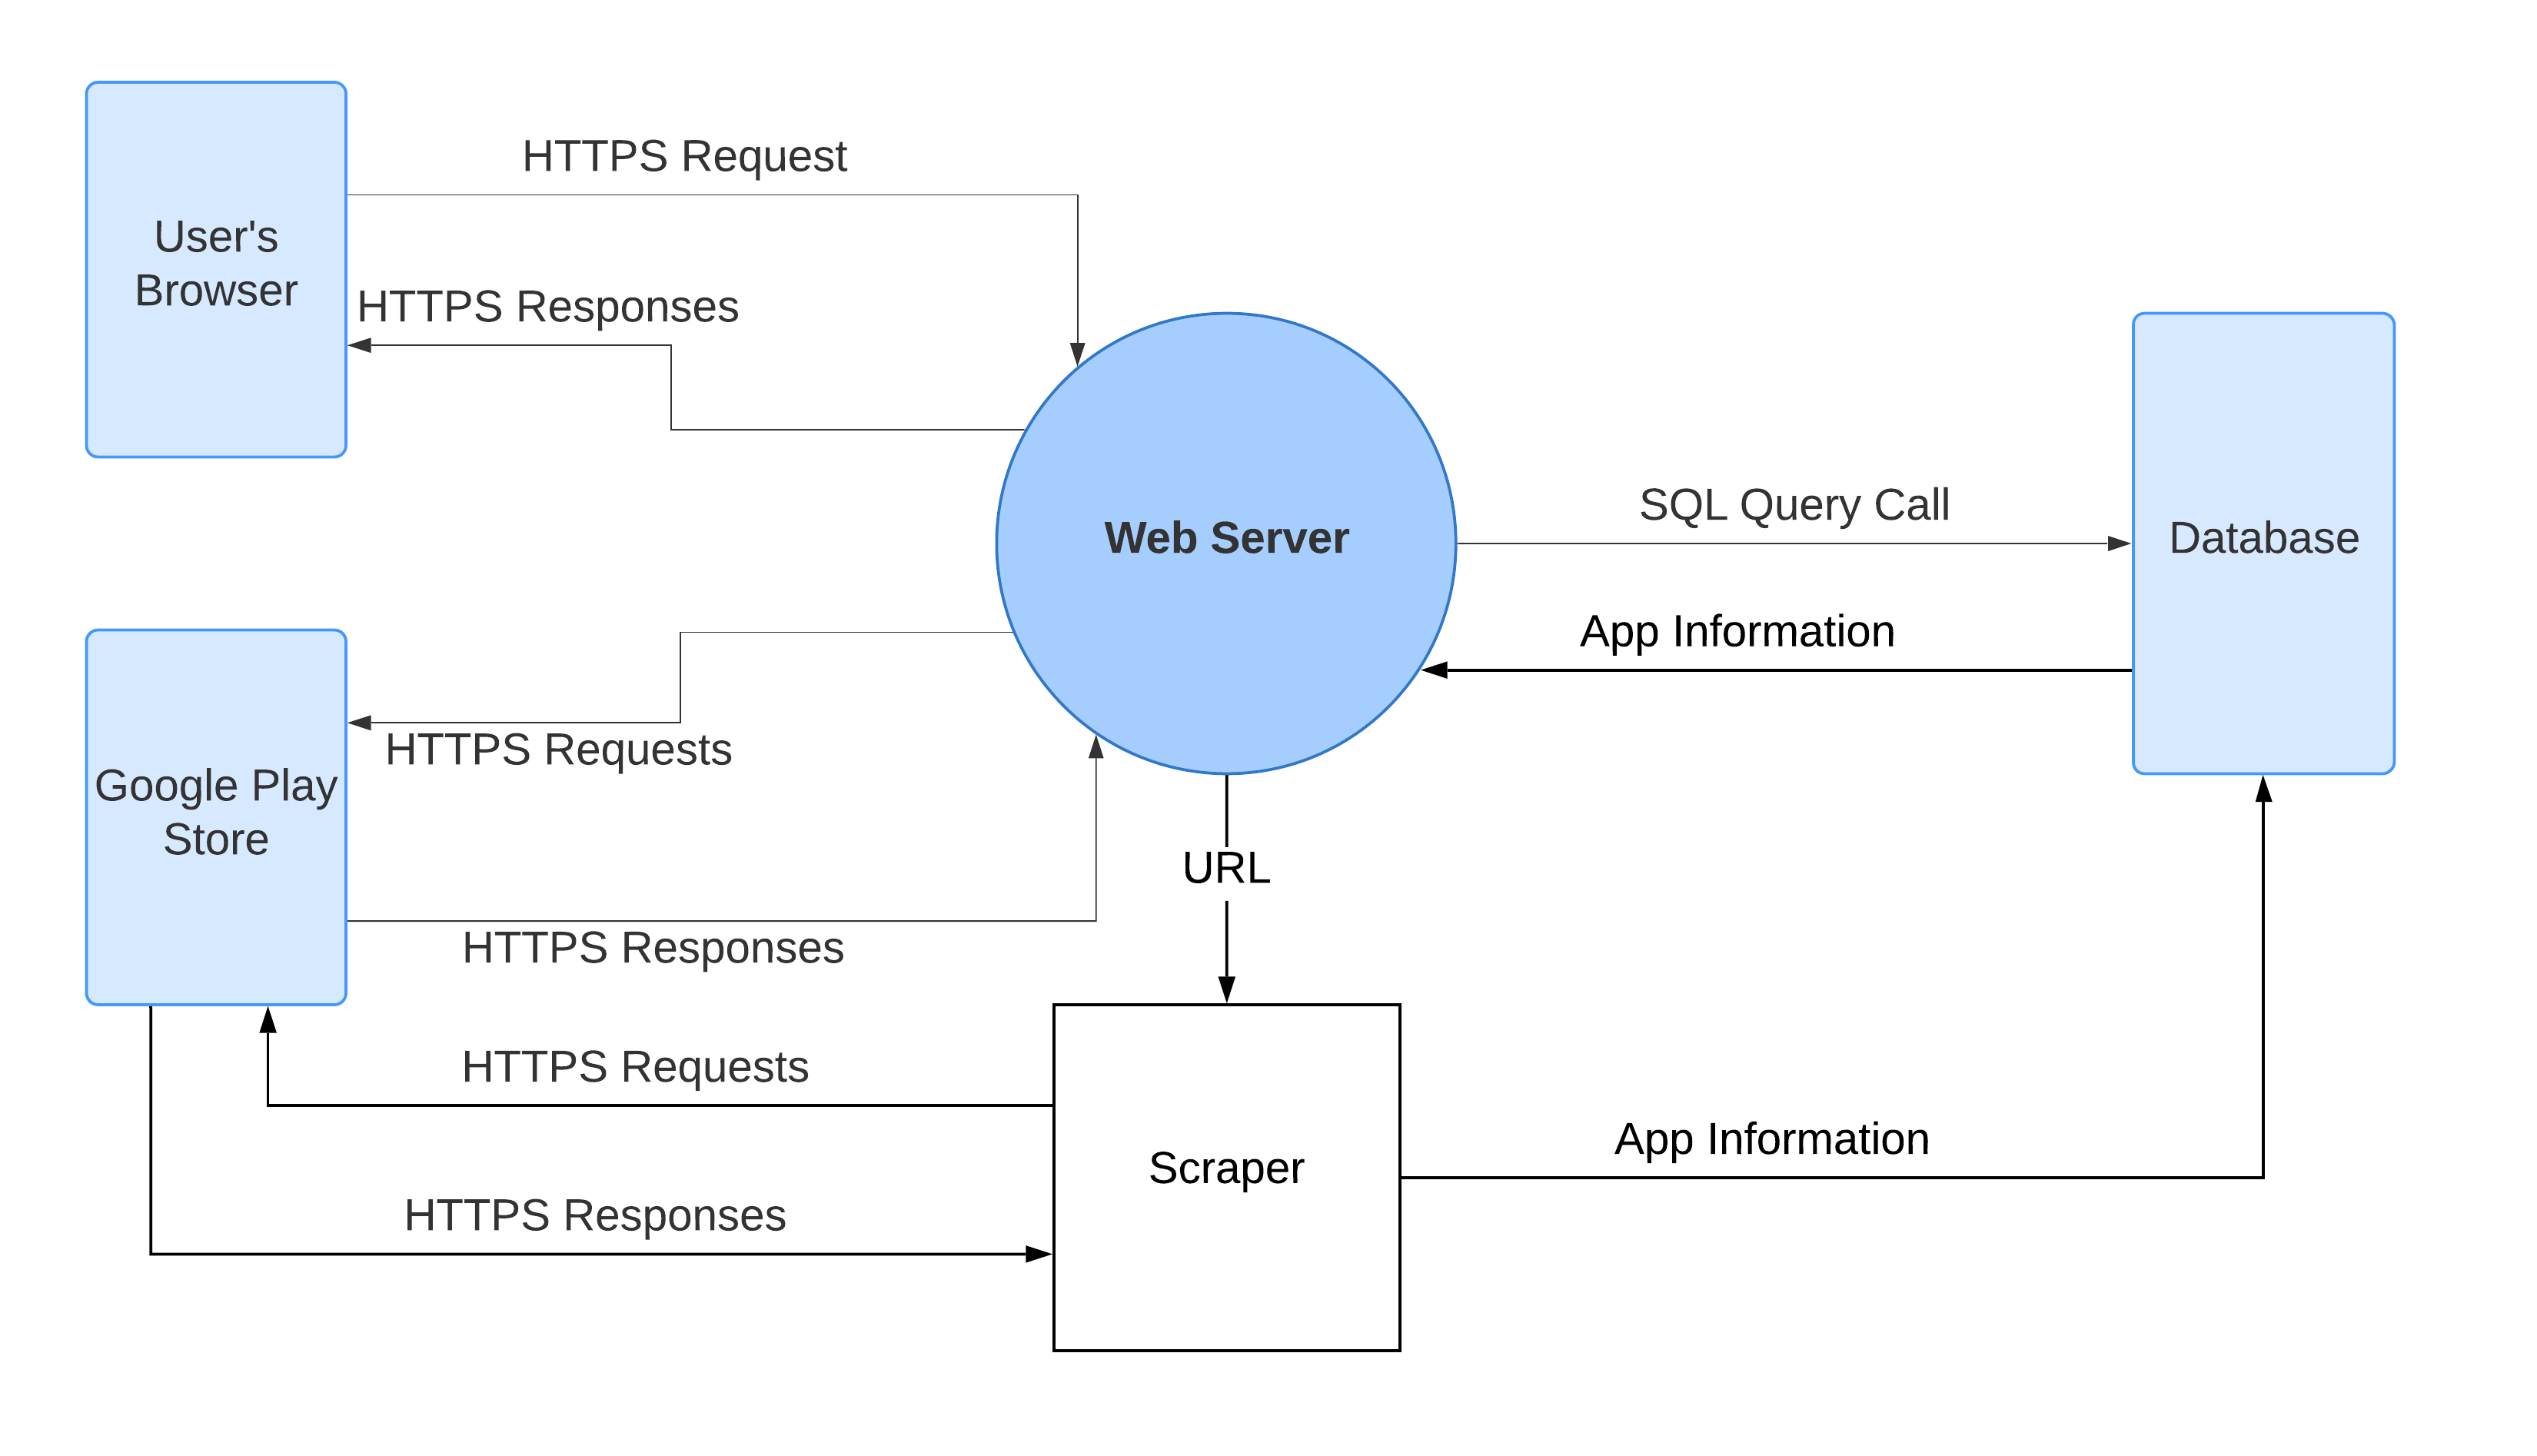
\includegraphics[width=1\textwidth]{Data_Flow_Diagram.png}
\caption{Data Flow Diagram}
\label{fig:Data_Flow}
\end{figure}

\subsection{Mitigate Denial-of-service Attack}
Denial-of-service Attack is a threat to our application. When facing a DOS threat, the victim may be attacked by a significant amount of incoming traffic from different sources so that the service of a website becomes unavailable. For example, an attacker might start a malicious activity by gathering the use of thousands of devices over the Internet to send a devastating number of unwanted packets to a website, which usually would be either large packets containing tons of data or sending large amount of small packets individually at the same time, making the website function much slower than usual or even out of service. For our product, it might not have to be a malicious activity from outside attackers but can also be that our website having an unexpected large number of users trying to search simultaneously, the server of our website might not be able to handle that.
Figure \ref{fig:dos} illustrates the attack tree .

In order to mitigate DOS attack, our team have come up with several possible solution which can be applied into our future development when building our website. One of them is that our application may impose a rate limit, for instance, an IP address can only send 10 search requests every 1 minute. If s/he reaches the limit, our website should show a warning. If s/he continues sending requests, we should block the IP through Linux firewall.

\begin{figure}[ht]
    \centering
    \begin{forest}
  for tree={
    draw,
    edge={-{Stealth[]}},
    l sep+=7.5pt,
    align=center,
  },
  [DOS Attack
    [Attack internally\\from the server
        [Gain access \\to the server, name=access-to-server]
    ]
    [Send massive requests\\from outside
        [Attacker gets\\many bots, tree angle=9mm]
        [server firewall\\is down]
            {\draw[->] () to[out=south west, in=south] (access-to-server);} % ()表示当前节点
    ]
    [Sends requests\\causing long execution
        [Find a bug in\\ our application]
    ]
  ]
\end{forest}

    \caption{Attack tree for DOS Attack}
    \label{fig:dos}
\end{figure}


\subsubsection{Prevent Arbitrary Code Execution}
We must not allow attackers to inject their code to our website and our website runs or sends the code to visitors to run. Figure \ref{fig:arbitrary-code-execution} illustrates the attack tree.

SQL Injection is a usually way to inject code. For example, our website has a search box and an attack may input some SQL update statement. If our database accidental executes the update statement, the database gets modified. If our website renders the injected data as HTML, it will execute on user's browser.

To prevent SQL injection, we use SQL parameterization when running SQL statements. In places where SQL parameterization is not supported, user input should be checked to ensure the security of data input. For example, single quotation marks, double quotation marks, colons and other characters should be converted or filtered.

What's more, it's possible that an attacker performs man-in-the-middle attack that hijacks the session between our server and Google Play. Google Play is using HTTPS so every time we scrape Google Play, we should check if the certificate is valid.

Our website needs to render app data as text instead of as HTML so that even if app data contains valid HTML, they will not execute on user's browser.

\begin{figure}[ht]
    \centering
    \begin{forest}
  for tree={
    draw, %框起来
    edge={-{Stealth[]}},
    l sep+=7.5pt, %vertical space between node and its parent.
    align=center,
  },
  [Run arbitrary code on our web page
    [Code injected to database, tree angle=9mm
        [Attacker gains\\direct access\\ to database]
        [The code\\ is from\\ Google Play
            [Attacker bypasses\\Google Play\\security check]
            [Man-in-the-middle\\attack on\\Google Play]
        ]
        [The code is\\from web search\\ interface
            [Database\\is writable, tree angle=12mm]
            [SQL\\paramertization\\failed]
        ]
    ]
    [Website treats\\the code as HTML]
  ]
\end{forest}
 \caption{Attack tree for arbitrary code execution}
   \label{fig:arbitrary-code-execution}
    
\end{figure}


\subsection{Prevent Cross-site request forgery (CSRF)}
It can steal or manipulate customer sessions and cookies, which can be used to impersonate a legitimate user, enabling hackers to view or change user records and execute transactions as that user.

Solution: 

Check the HTTP header refer information - After the Server receives the request, it can check the header and accept only the request from the local domain and ignore the request from the external domain.

Determine the type of HTTP request - Use \code{request.getMethod()} to determine whether the request is posted.

\subsection{Support HTTPS Communication}
When we develop the application, we test it with http://localhost. We shall make sure the application support HTTPS communication as our production server will enable HTTPS. 

In addition, we may enable OCSP Stapling. %补充一下

We may not enable HTTP Strict Transport Security because it requires our website to always have a valid certificate. We don't have enough manpower to maintain it.

\section{Lessons Learned}
\subsection{When designing the system}
When designing a software, we should always think of potential security issues beforehand by performing risks analysis. With the tools and principles we have learned in class, one can always get a general idea of the problems that a project might be facing. The secure design principles suggest that we follow an economy of mechanism, have fail-safe defaults, complete mediation, least privilege, psychological acceptability, compromise recording, defense in depth, design for updating, open design, promote privacy and be reluctant to trust. The most fundamental part of our team's understanding is that one should not do extra work on what we don’t need and grant least amount of access as Economy of mechanism and fail-safe defaults suggest. We should default to lack of access. It’s convenient to grant all access without really considering their functionalities individually but it’s very dangerous to do so since malicious hackers can easily attack the product by installing and executing malicious scripts. Forgetting to grant access may cause errors but it keeps the software secure. Similar reasons for granting least privilege, a secure system should give the minimum access and permissions. For example, since our web server interacts with a database, we don’t want the server to have full access of the database in case the server is hacked and we also don’t want users to have access to gain information from database for privacy concerns. For now our database does not store any type of personal information so we should be safe from that but in case we have account access for users, we should always think of this issue beforehand. Also when designing a product, it’s essential to find a balance between security and a better user experience. The key point is that we want our website to be convenient for users and making it too complicated would lead to the loss of customers.
\subsection{While Secure Coding}
While coding, always think of major problems areas for security purposes. It’s important to keep in mind these problems in mind and scan through the major problem areas during the development of the system. For example, since we ask users for keyword inputs for searching, we were thinking if we would have buffer overflow attack when users inputs are too long. However, as we did some research we found out that the latest version of the 3.3.4 python is safe from buffer overflow with the vulnerability has been patched.
\subsection{When Evaluating the Security of the System}
After going through the above process and when it comes to evaluating, we are able to narrow down the scope to specific problem areas based on individual types of the design since different types of projects may have different kinds of security issues. For example, our project does not have problems with encryption and decryption but we have problems such as SQL injections since we ask users for input keywords. Therefore, for efficient evaluating, we should focus more on the higher potential problems regarding on database. However, we always need to keep an eye on the general problems like error handling and checking return codes since all programs have a potential risks of making mistakes on these areas. When testing the system, it's also useful to consider edge cases like running on an unprivileged mode and check if it can do work on higher privilege mode. In addition, it's helpful to create a list of a structure of the code to check if it creates any potential bugs such as problems caused by race conditions. Sometimes looking all the problems on our own is not enough and testing tools can be a great help too.
\section{Work Breakdown}
Shuhua Zhan - responsible for lessons learned section of the report and participated in code review. In the project, participated in element \code{app\_icon}, fixed problem when no results find in google play website and improved the user interface of the website.


\newcommand{\citeWeb}[3]{#1, \url{#2}, Retrieved #3.}


\end{document}